\documentclass[12pt, a4paper]{article}

\usepackage[utf8]{inputenc}
\usepackage[T1]{fontenc}
\usepackage[spanish]{babel}
\usepackage[margin=2.5cm]{geometry}
\usepackage{booktabs}
\usepackage{tabularx}
\usepackage{array}
\usepackage{listings}
\usepackage{xcolor}
\usepackage{hyperref}
\usepackage{graphicx}
\usepackage{float}
\usepackage{parskip}
\usepackage{titlesec}
\usepackage{fancyhdr}
\usepackage{enumitem}
\usepackage{setspace}

\definecolor{codebackground}{rgb}{0.95,0.95,0.95}
\definecolor{codekeyword}{rgb}{0.13,0.29,0.53}
\definecolor{codecomment}{rgb}{0.25,0.5,0.37}
\definecolor{codestring}{rgb}{0.63,0.13,0.13}
\definecolor{accentblue}{RGB}{30,90,160}
\definecolor{darkbg}{RGB}{40,44,52}

\lstset{
  backgroundcolor=\color{codebackground},
  basicstyle=\ttfamily\small,
  keywordstyle=\color{codekeyword}\bfseries,
  commentstyle=\color{codecomment}\itshape,
  stringstyle=\color{codestring},
  breaklines=true,
  frame=single,
  rulecolor=\color{gray!40},
  numbers=none,
  xleftmargin=6pt,
  xrightmargin=6pt,
  aboveskip=8pt,
  belowskip=8pt,
  language=Python,
  showstringspaces=false,
  tabsize=4,
  literate={á}{{\'a}}1 {é}{{\'e}}1 {í}{{\'i}}1 {ó}{{\'o}}1 {ú}{{\'u}}1
           {Á}{{\'A}}1 {É}{{\'E}}1 {Í}{{\'I}}1 {Ó}{{\'O}}1 {Ú}{{\'U}}1
           {ñ}{{\~n}}1 {Ñ}{{\~N}}1,
}

\pagestyle{fancy}
\fancyhf{}
\rhead{\small Manual de Programación -- Actividad 7}
\lhead{\small dperez37}
\rfoot{\small\thepage}
\renewcommand{\headrulewidth}{0.4pt}
\setlength{\headheight}{15pt}

\hypersetup{colorlinks=true, linkcolor=accentblue, urlcolor=accentblue}

\titleformat{\section}{\large\bfseries\color{accentblue}}{}{0em}{}[\titlerule]
\titleformat{\subsection}{\normalsize\bfseries}{}{0em}{}

% columna de tabla con ancho fijo y wrap
\newcolumntype{L}[1]{>{\raggedright\arraybackslash}p{#1}}

\begin{document}

% ── Portada ───────────────────────────────────────────────────────────────────
\begin{titlepage}
  \centering
  \vspace*{3cm}
  {\Large\bfseries Universidad de La Salle\par}
  \vspace{0.3cm}
  {\normalsize Ciencias de Datos\par}
  \vspace{2.5cm}
  \rule{0.6\linewidth}{1pt}\par\vspace{1cm}
  {\LARGE\bfseries Actividad 7: Sistema CRUD GAD-7\par}
  \vspace{0.4cm}
  {\normalsize Lenguaje de Programación II\par}
  \vspace{1cm}
  \rule{0.6\linewidth}{1pt}\par\vspace{2.5cm}
  {\large\bfseries Diunis Pérez\par}
  \vspace{0.3cm}
  {\small dperez37 \quad|\quad rama: \texttt{dev\_dperez37}\par}
  \vspace{0.3cm}
  {\small 24 de mayo de 2026\par}
  \vspace{1cm}
  {\small\textbf{Repositorio:} \url{https://github.com/dperezt18/Actividad7}\par}
\end{titlepage}

\newpage\setcounter{page}{1}

% ══════════════════════════════════════════════════════════════════════════════
\section{Descripción General}

Este proyecto implementa un sistema \textbf{CRUD} completo sobre la entidad
\textbf{CuestionarioGAD7}, el cuestionario clínico estandarizado de detección de
trastorno de ansiedad generalizada (\textit{Generalized Anxiety Disorder~7}),
aplicado a estudiantes universitarios.

El sistema está desarrollado en \textbf{Python~3.13} aplicando principios SOLID,
Clean Code y PEP~8, con persistencia en formato \textbf{JSON} (requerida por la
actividad) y soporte adicional en \textbf{MySQL Workbench}. La interfaz de
usuario es en consola (CLI).

\vspace{0.5em}
\begin{tabular}{L{3.5cm} L{10.5cm}}
  \toprule
  \textbf{Módulo} & \textbf{Descripción} \\
  \midrule
  Modelo &
    Clases \texttt{CuestionarioGAD7} y \texttt{Respuesta}: encapsulan los datos,
    validan entradas (valor 0--3 por ítem) y calculan puntaje y nivel de severidad. \\[6pt]
  Repositorio DAO &
    Interfaz \texttt{IRepository[T]} (ABC) con 5 métodos CRUD. Implementaciones
    concretas en JSON y MySQL. \\[6pt]
  Servicio &
    \texttt{GAD7Service}: orquesta la lógica de negocio y valida completitud del
    cuestionario antes de persistir. \\[6pt]
  Vista &
    \texttt{MenuPrincipal}: interfaz CLI con menú numerado y validaciones inmediatas. \\[6pt]
  Excepciones &
    Jerarquía \texttt{AppError} $\rightarrow$ \texttt{EntidadNoEncontradaError},
    \texttt{CuestionarioIncompletoError}, \texttt{ValorFueraDeRangoError}. \\
  \bottomrule
\end{tabular}

% ══════════════════════════════════════════════════════════════════════════════
\section{Análisis y Diseño}

Antes de escribir código se identificaron los conceptos de la unidad y cómo
aplicarlos al problema de gestión de cuestionarios GAD-7:

\vspace{0.5em}
\begin{tabular}{L{4cm} L{10cm}}
  \toprule
  \textbf{Concepto de la unidad} & \textbf{Decisión de diseño} \\
  \midrule
  Patrón MVC &
    Se separó presentación (\texttt{MenuPrincipal}), lógica de negocio
    (\texttt{GAD7Service}) y datos (\texttt{CuestionarioGAD7}). \\[6pt]
  Patrón DAO/Repository &
    Se definió \texttt{IRepository[T]} como interfaz abstracta. El servicio
    nunca accede directamente a archivos ni a la BD. \\[6pt]
  Principios SOLID &
    Cada clase tiene una responsabilidad única. El repositorio es
    intercambiable sin modificar el servicio. \\[6pt]
  Persistencia JSON &
    Requerida por la actividad. El archivo \texttt{cuestionarios\_gad7.json}
    se crea automáticamente si no existe. \\[6pt]
  Persistencia MySQL &
    Añadida como mejora. Permite consultar los datos desde MySQL Workbench
    con SQL estándar sin cambiar ninguna capa del sistema. \\
  \bottomrule
\end{tabular}

% ══════════════════════════════════════════════════════════════════════════════
\section{Estructura del Proyecto}

\begin{lstlisting}[language={}, backgroundcolor=\color{darkbg},
                   basicstyle=\ttfamily\footnotesize\color{white},
                   frame=single, rulecolor=\color{darkbg}]
Actividad7/
|-- main.py                          <- Punto de entrada (composition root)
|-- requirements.txt
|-- app/
|   |-- exceptions.py                <- Jerarquia de excepciones de dominio
|   |-- interfaces/
|   |   `-- i_repository.py          <- Contrato ABC con 5 metodos CRUD
|   |-- models/
|   |   |-- cuestionario_gad7.py     <- Entidad principal (dataclass)
|   |   |-- respuesta.py             <- Entidad Respuesta (dataclass)
|   |   `-- estado_riesgo.py         <- Enum: NORMAL / LEVE / MODERADO / SEVERO
|   |-- repositories/
|   |   |-- gad7_repository_json.py  <- Implementacion DAO -> JSON
|   |   `-- gad7_repository_mysql.py <- Implementacion DAO -> MySQL Workbench
|   |-- services/
|   |   `-- gad7_service.py          <- Logica de negocio (CRUD)
|   `-- ui/
|       |-- menu.py                  <- CLI interactivo
|       `-- mensajes.py              <- Constantes de texto
|-- data/
|   `-- cuestionarios_gad7.json      <- Almacenamiento persistente JSON
`-- tests/
    `-- test_gad7.py                 <- 29 pruebas unitarias con pytest
\end{lstlisting}

% ══════════════════════════════════════════════════════════════════════════════
\section{Patrones de Diseño: MVC y DAO/Repository}

\subsection{Patrón MVC (Model -- View -- Controller)}

\textbf{Definición formal:} MVC divide la aplicación en tres componentes con
responsabilidades bien delimitadas. El \textit{Modelo} gestiona los datos y la
lógica de dominio sin conocer la presentación; la \textit{Vista} presenta la
información sin contener lógica de negocio; el \textit{Controlador/Servicio}
recibe las acciones del usuario y las delega al Modelo. El objetivo es lograr
bajo acoplamiento y alta cohesión entre las capas.
\textit{(Gamma et al., ``Design Patterns'', 1994.)}

\vspace{0.5em}
\begin{tabularx}{\linewidth}{L{1.8cm} X X}
  \toprule
  \textbf{Rol} & \textbf{Clase / Archivo} & \textbf{Responsabilidad} \\
  \midrule
  Model &
    \texttt{CuestionarioGAD7}\newline
    {\small\texttt{models/cuestionario\_gad7.py}} &
    Valida datos, calcula puntaje y clasifica severidad. No conoce la vista. \\[6pt]
  View &
    \texttt{MenuPrincipal}\newline
    {\small\texttt{ui/menu.py}} &
    Muestra menús y lee input. No contiene lógica de negocio. \\[6pt]
  Service &
    \texttt{GAD7Service}\newline
    {\small\texttt{services/gad7\_service.py}} &
    Orquesta el CRUD, valida y delega al repositorio. \\
  \bottomrule
\end{tabularx}

\subsection{Patrón DAO / Repository}

\textbf{Definición formal:} El patrón \textit{Data Access Object} (DAO) define
una interfaz que abstrae el acceso a una fuente de datos. Toda la lógica de
persistencia queda en el objeto concreto; el resto del sistema depende únicamente
del contrato abstracto, sin importar si los datos están en un archivo o en una BD.
\textit{(Fowler, ``Patterns of Enterprise Application Architecture'', 2002.)}

\vspace{0.5em}
\begin{tabularx}{\linewidth}{L{3cm} L{4.5cm} X}
  \toprule
  \textbf{Componente} & \textbf{Clase} & \textbf{Rol} \\
  \midrule
  Contrato abstracto &
    \texttt{IRepository[T]} &
    ABC genérica con 5 métodos: \texttt{crear}, \texttt{listar},
    \texttt{buscar\_por\_codigo}, \texttt{actualizar}, \texttt{eliminar}. \\[6pt]
  Implementación JSON &
    \texttt{GAD7RepositoryJSON} &
    Persiste con \texttt{json.load}/\texttt{json.dump}. Crea el archivo
    automáticamente si no existe. \\[6pt]
  Implementación MySQL &
    \texttt{GAD7RepositoryMySQL} &
    Persiste en MySQL Workbench. Crea la BD y tabla automáticamente. \\[6pt]
  Consumidor &
    \texttt{GAD7Service} &
    Recibe \texttt{IRepository} por inyección de dependencias. Nunca
    instancia el repositorio directamente. \\
  \bottomrule
\end{tabularx}

% ══════════════════════════════════════════════════════════════════════════════
\section{Principios SOLID}

\begin{tabular}{L{3.5cm} L{3.5cm} L{7cm}}
  \toprule
  \textbf{Principio} & \textbf{Definición} & \textbf{Evidencia en el proyecto} \\
  \midrule
  S — Single Responsibility &
    Cada clase tiene una única razón para cambiar. &
    \texttt{CuestionarioGAD7} solo modela datos; \texttt{GAD7RepositoryJSON}
    solo persiste; \texttt{MenuPrincipal} solo presenta. \\[8pt]
  O — Open/Closed &
    Abierto para extensión, cerrado para modificación. &
    Para agregar otro motor de BD basta crear una nueva clase que implemente
    \texttt{IRepository}, sin tocar el servicio ni los modelos. \\[8pt]
  L — Liskov Substitution &
    Las subclases sustituyen a su base sin romper el comportamiento. &
    Los tests usan \texttt{MagicMock()} como sustituto del repositorio real
    y el servicio funciona exactamente igual. \\[8pt]
  I — Interface Segregation &
    Interfaces pequeñas y específicas. &
    \texttt{IRepository} define solo los 5 métodos del dominio GAD-7, sin
    métodos de otras entidades del sistema. \\[8pt]
  D — Dependency Inversion &
    Depender de abstracciones, no de implementaciones concretas. &
    \texttt{GAD7Service.\_\_init\_\_(self, repositorio: IRepository[...])}. El
    único lugar con instancias concretas es \texttt{main.py}. \\
  \bottomrule
\end{tabular}

% ══════════════════════════════════════════════════════════════════════════════
\section{Sistema GAD-7 — CRUD}

\subsection{Clasificación de Severidad}

El puntaje total es la suma de las 7 respuestas (valor 0--3 por ítem; máximo 21).
La clasificación sigue los umbrales clínicos estándar del GAD-7:

\vspace{0.5em}
\begin{tabular}{L{4cm} L{4cm} L{6cm}}
  \toprule
  \textbf{Nivel} & \textbf{Puntaje} & \textbf{Constante en código} \\
  \midrule
  Normal   & 0 -- 4  & \texttt{puntaje < UMBRAL\_LEVE = 5} \\[4pt]
  Leve     & 5 -- 9  & \texttt{UMBRAL\_LEVE = 5} \\[4pt]
  Moderado & 10 -- 14 & \texttt{UMBRAL\_MODERADO = 10} \\[4pt]
  Severo   & 15 -- 21 & \texttt{UMBRAL\_SEVERO = 15} \\
  \bottomrule
\end{tabular}

\newpage
\subsection{Fragmentos de Código Clave}

\textbf{Modelo — clasificación de severidad:}
\begin{lstlisting}
@dataclass
class CuestionarioGAD7:
    codigo_estudiante: str
    respuestas: List[Respuesta] = field(default_factory=list)
    id: str = field(default_factory=lambda: str(uuid.uuid4()))
    fecha_aplicacion: datetime = field(default_factory=datetime.now)

    @property
    def puntaje_total(self) -> int:
        return sum(r.valor for r in self.respuestas)

    def clasificar_severidad(self) -> EstadoRiesgo:
        puntaje = self.puntaje_total
        if puntaje >= UMBRAL_SEVERO:   return EstadoRiesgo.SEVERO
        if puntaje >= UMBRAL_MODERADO: return EstadoRiesgo.MODERADO
        if puntaje >= UMBRAL_LEVE:     return EstadoRiesgo.LEVE
        return EstadoRiesgo.NORMAL
\end{lstlisting}

\textbf{Interfaz DAO — contrato genérico:}
\begin{lstlisting}
class IRepository(ABC, Generic[T]):
    @abstractmethod
    def crear(self, entidad: T) -> T: ...
    @abstractmethod
    def listar(self) -> List[T]: ...
    @abstractmethod
    def buscar_por_codigo(self, codigo: str) -> Optional[T]: ...
    @abstractmethod
    def actualizar(self, entidad: T) -> T: ...
    @abstractmethod
    def eliminar(self, codigo: str) -> None: ...
\end{lstlisting}

\textbf{Servicio — inyección de dependencias:}
\begin{lstlisting}
class GAD7Service:
    def __init__(self, repositorio: IRepository[CuestionarioGAD7]) -> None:
        self._repo = repositorio  # abstraccion, no JSON ni MySQL directamente

    def crear_cuestionario(self, codigo: str, respuestas: List[Respuesta]):
        cuestionario = CuestionarioGAD7(codigo_estudiante=codigo,
                                        respuestas=respuestas)
        if not cuestionario.validar():
            raise CuestionarioIncompletoError(
                "Debe tener exactamente 7 respuestas.")
        return self._repo.crear(cuestionario)
\end{lstlisting}

% ══════════════════════════════════════════════════════════════════════════════
\section{Persistencia en MySQL Workbench}

Se utilizó MySQL Workbench como base de datos relacional adicional al JSON
requerido. La decisión de usar MySQL se basa en que permite consultar los
cuestionarios con SQL estándar, visualizar los datos en tablas y escalar el
sistema a producción sin cambiar ninguna capa del código.

El repositorio \texttt{GAD7RepositoryMySQL} crea automáticamente la base de
datos \texttt{gad7\_db} y la tabla \texttt{cuestionarios\_gad7} si no existen,
lo que facilita la primera ejecución sin configuración manual.

\begin{figure}[H]
  \centering
  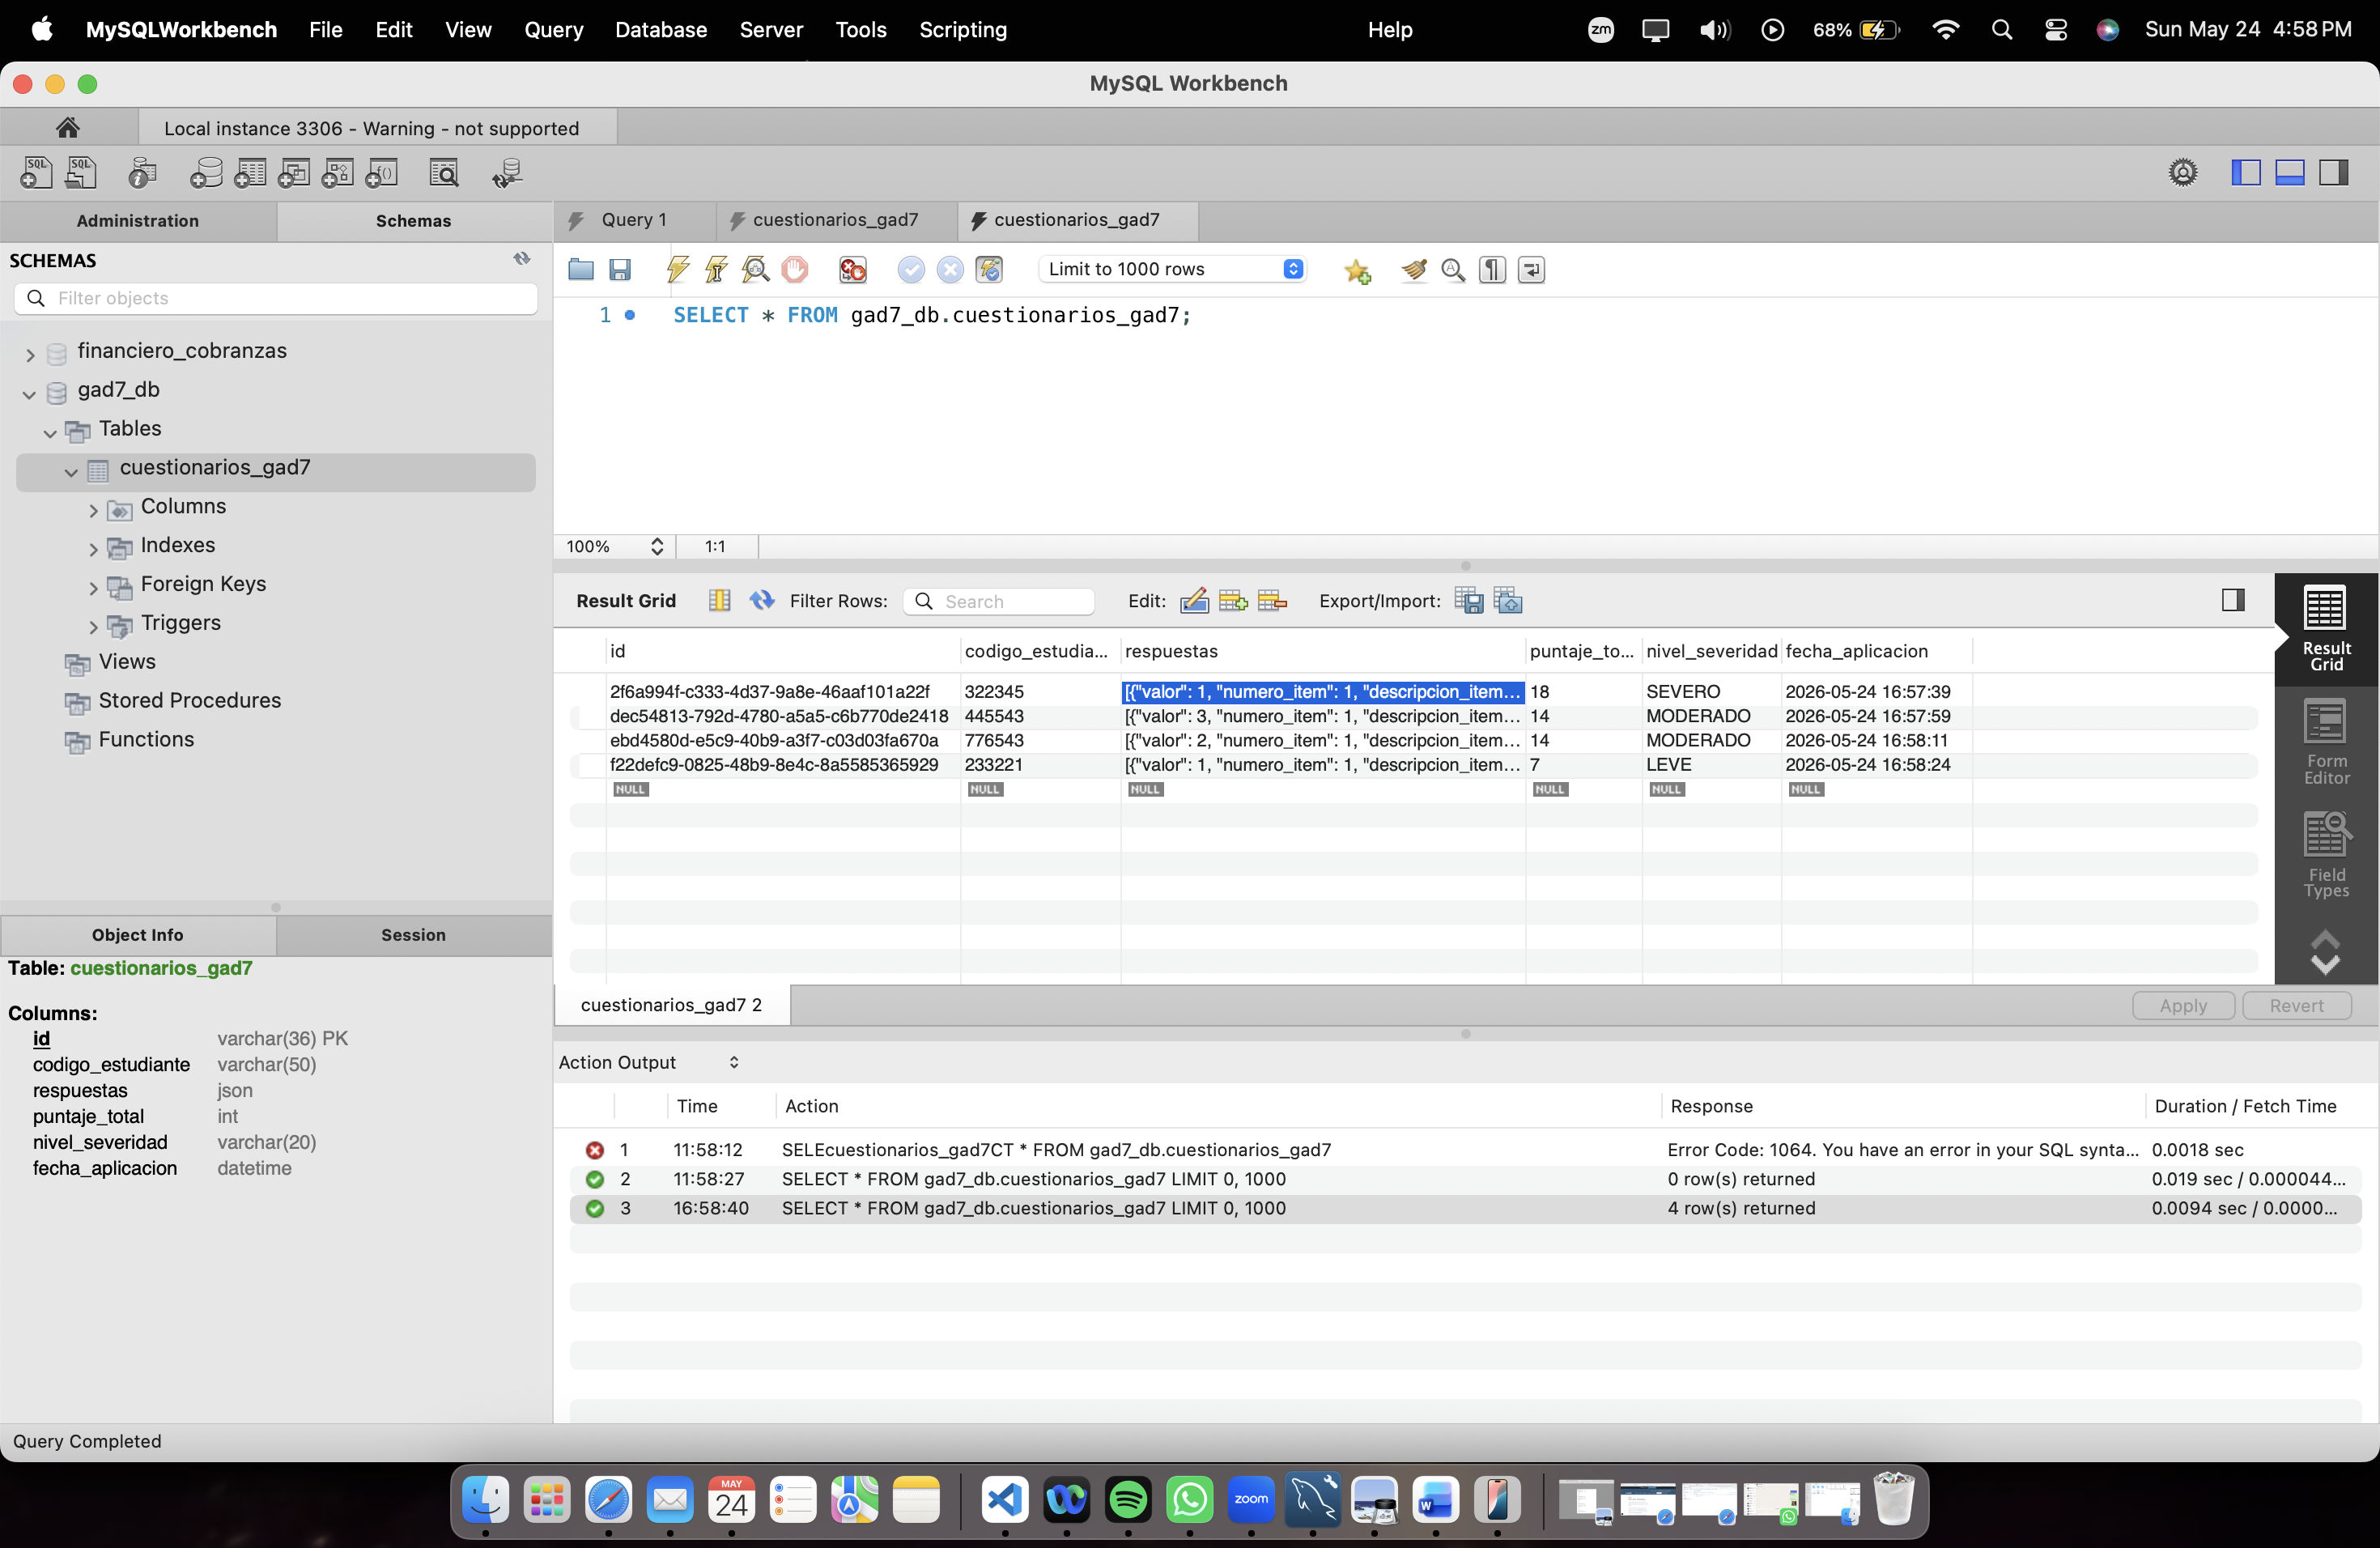
\includegraphics[width=\linewidth]{sql.png}
  \caption{Tabla \texttt{cuestionarios\_gad7} en MySQL Workbench con registros reales}
\end{figure}

% ══════════════════════════════════════════════════════════════════════════════
\section{Pruebas Unitarias}

\subsection{Estrategia}

Se diseñaron \textbf{29 casos de prueba} con \texttt{pytest} distribuidos en 4
clases, cubriendo: validación de entrada, todos los umbrales de severidad como
\textit{edge cases}, lógica del servicio con repositorio simulado
(\texttt{MagicMock}) y pruebas de integración del repositorio JSON con archivos
temporales (\texttt{tmp\_path}).

\subsection{Resumen de Resultados}

\begin{tabularx}{\linewidth}{X r r r l}
  \toprule
  \textbf{Clase de prueba} & \textbf{Tests} & \textbf{Fallos} & \textbf{Errores} & \textbf{Resultado} \\
  \midrule
  \texttt{TestRespuesta}                     &  6 & 0 & 0 & \checkmark\ PASSED \\
  \texttt{TestCuestionarioGAD7}              & 11 & 0 & 0 & \checkmark\ PASSED \\
  \texttt{TestGAD7Service}                   &  7 & 0 & 0 & \checkmark\ PASSED \\
  \texttt{TestGAD7RepositoryJSONIntegracion} &  5 & 0 & 0 & \checkmark\ PASSED \\
  \midrule
  \textbf{TOTAL} & \textbf{29} & \textbf{0} & \textbf{0} & \checkmark\ \textbf{OK} \\
  \bottomrule
\end{tabularx}

\subsection{Edge Cases Destacados}

\begin{tabularx}{\linewidth}{X L{5.5cm}}
  \toprule
  \textbf{Test} & \textbf{Qué verifica} \\
  \midrule
  {\small\texttt{test\_clasificar\_normal\_puntaje\_4}}           & Puntaje 4 sigue siendo NORMAL \\[4pt]
  {\small\texttt{test\_clasificar\_leve\_umbral\_exacto\_5}}      & Puntaje 5 es el primer LEVE \\[4pt]
  {\small\texttt{test\_clasificar\_moderado\_umbral\_exacto\_10}} & Puntaje 10 es el primer MODERADO \\[4pt]
  {\small\texttt{test\_clasificar\_severo\_umbral\_exacto\_15}}   & Puntaje 15 es el primer SEVERO \\[4pt]
  {\small\texttt{test\_clasificar\_severo\_puntaje\_maximo\_21}}  & Puntaje máximo sigue siendo SEVERO \\[4pt]
  {\small\texttt{test\_valor\_4\_lanza\_error}}                   & Respuesta con valor 4 lanza \texttt{ValueError} \\[4pt]
  {\small\texttt{test\_valor\_negativo\_lanza\_error}}            & Respuesta negativa lanza \texttt{ValueError} \\[4pt]
  {\small\texttt{test\_eliminar\_inexistente\_lanza\_error}}      & Eliminar ID inexistente lanza error \\
  \bottomrule
\end{tabularx}

\subsection{Captura de Ejecución}

\begin{figure}[H]
  \centering
  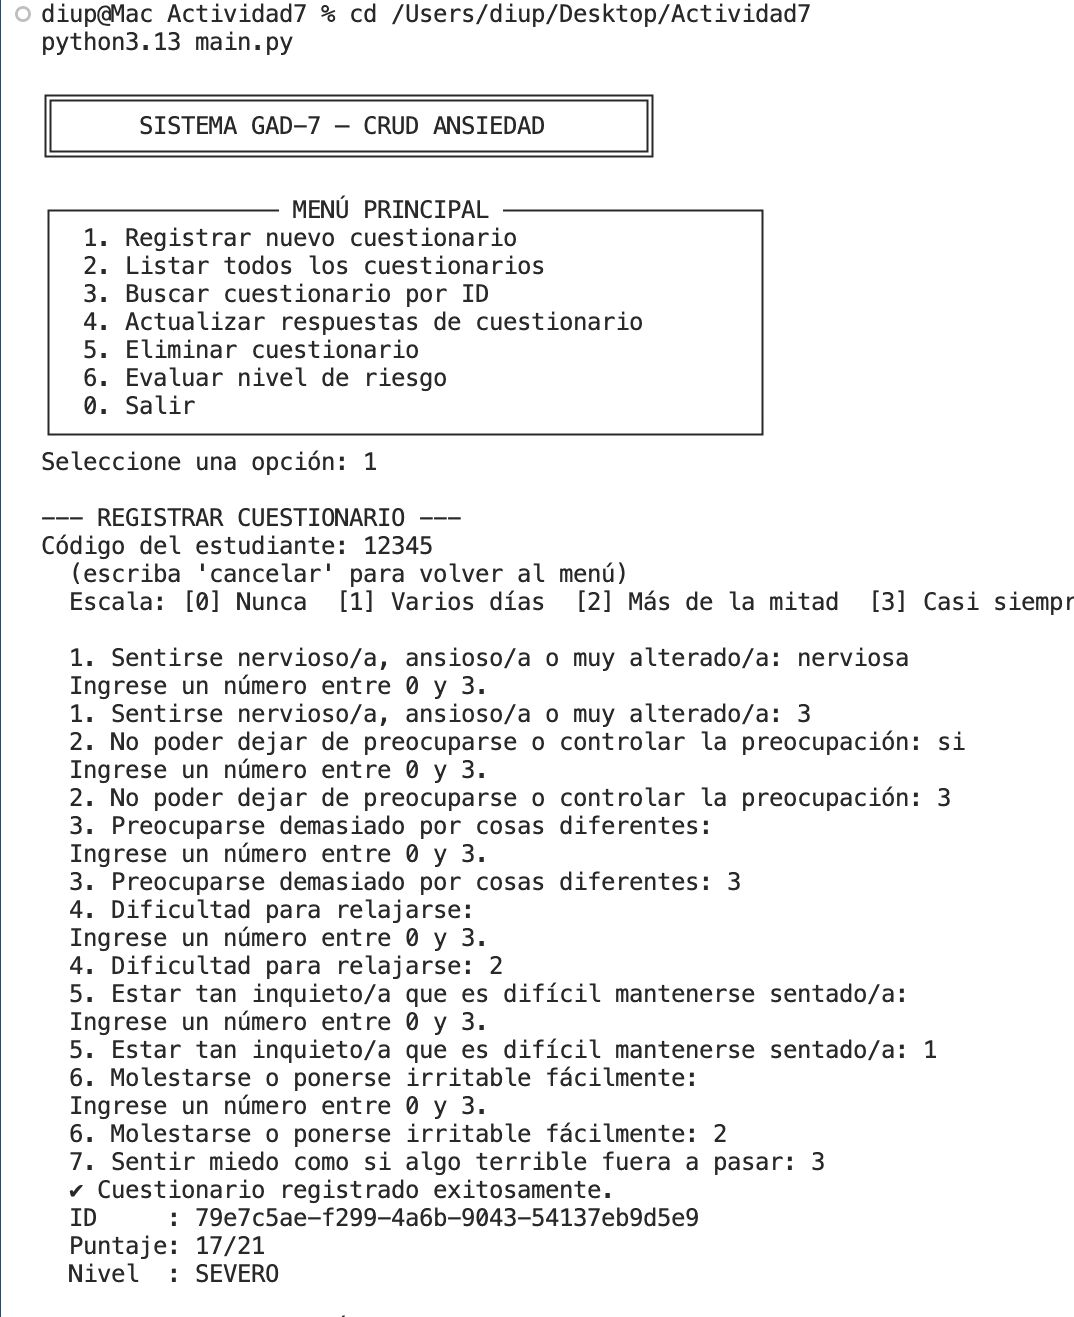
\includegraphics[width=\linewidth]{Prueba.png}
  \caption{Ejecución de las 29 pruebas unitarias — todas pasando}
\end{figure}

\newpage
% ══════════════════════════════════════════════════════════════════════════════
\section{Ejecución del Programa}

\begin{lstlisting}[language=bash]
# Instalar dependencias
pip install -r requirements.txt

# Ejecutar pruebas
python3.13 -m pytest tests/test_gad7.py -v

# Ejecutar el programa (modo JSON)
# En main.py: USE_MYSQL = False
python3.13 main.py

# Ejecutar el programa (modo MySQL Workbench)
# En main.py: USE_MYSQL = True
python3.13 main.py
\end{lstlisting}

\vspace{1em}\hrule\vspace{0.5em}
{\small Actividad 7 -- Lenguaje de Programación II -- Universidad de La Salle -- 2026 -- dperez37}

\end{document}
